\section{Data Preparation}\label{Sec:Data Preparation}

Even though the scraped data has already been partially .... from ...., not all information is necessary for our analysis and some feature engineering is needed.

Moreover, the spatial data from the downloaded shapefiles also requires to be reprocessed.

\subsection{Berlin neighbourhoods and districts}


Berlin consists of 96 neighbourhoods (Ortsteile), which are grouped into 12 districts (Bezirke).

\begin{table}[H]
\centering
\begin{tabular}{ll}
  \hline \hline
Neighbourhood & District \\ 
  \hline
Charlottenburg & Charlottenburg-Wilmersdorf \\ 
  Wilmersdorf & Charlottenburg-Wilmersdorf \\ 
  Grunewald & Charlottenburg-Wilmersdorf \\ 
  Westend & Charlottenburg-Wilmersdorf \\ 
  Schmargendorf & Charlottenburg-Wilmersdorf \\ 
  Charlottenburg-Nord & Charlottenburg-Wilmersdorf \\ 
  Halensee & Charlottenburg-Wilmersdorf \\ 
  Friedrichshain & Friedrichshain-Kreuzberg \\ 
  Kreuzberg & Friedrichshain-Kreuzberg \\ 
  Friedrichsfelde & Lichtenberg \\ 
  Karlshorst & Lichtenberg \\ 
  Malchow & Lichtenberg \\ 
  Wartenberg & Lichtenberg \\ 
  Falkenberg & Lichtenberg \\ 
  Fennpfuhl & Lichtenberg \\ 
  Lichtenberg & Lichtenberg \\ 
  Neu-Hohenschönhausen & Lichtenberg \\ 
  Alt-Hohenschönhausen & Lichtenberg \\ 
  Rummelsburg & Lichtenberg \\ 
  Marzahn & Marzahn-Hellersdorf \\ 
  Biesdorf & Marzahn-Hellersdorf \\ 
  Kaulsdorf & Marzahn-Hellersdorf \\ 
  Mahlsdorf & Marzahn-Hellersdorf \\ 
  Hellersdorf & Marzahn-Hellersdorf \\ 
  Mitte & Mitte \\ 
  Moabit & Mitte \\ 
  Hansaviertel & Mitte \\ 
  Gesundbrunnen & Mitte \\ 
  Tiergarten & Mitte \\ 
  Wedding & Mitte \\ 
  Buckow & Neukölln \\ 
  Buckow & Neukölln \\ 
  Gropiusstadt & Neukölln \\ 
  Neukölln & Neukölln \\ 
  Britz & Neukölln \\ 
  Rudow & Neukölln \\ 
  Blankenfelde & Pankow \\ 
  Buch & Pankow \\ 
  Wilhelmsruh & Pankow \\ 
  Prenzlauer Berg & Pankow \\ 
  Weißensee & Pankow \\ 
  Blankenburg & Pankow \\ 
  Heinersdorf & Pankow \\ 
  Karow & Pankow \\ 
  Stadtrandsiedlung Malchow & Pankow \\ 
  Pankow & Pankow \\ 
  Französisch Buchholz & Pankow \\ 
  Niederschönhausen & Pankow \\ 
  Rosenthal & Pankow \\ 
  Konradshöhe & Reinickendorf \\ 
  Tegel & Reinickendorf \\ 
  Märkisches Viertel & Reinickendorf \\ 
  Hermsdorf & Reinickendorf \\ 
  Borsigwalde & Reinickendorf \\ 
  Lübars & Reinickendorf \\ 
  Reinickendorf & Reinickendorf \\ 
  Heiligensee & Reinickendorf \\ 
  Frohnau & Reinickendorf \\ 
  Waidmannslust & Reinickendorf \\ 
  Wittenau & Reinickendorf \\ 
  Gatow & Spandau \\ 
  Kladow & Spandau \\ 
  Falkenhagener Feld & Spandau \\ 
  Wilhelmstadt & Spandau \\ 
  Spandau & Spandau \\ 
  Haselhorst & Spandau \\ 
  Siemensstadt & Spandau \\ 
  Staaken & Spandau \\ 
  Hakenfelde & Spandau \\ 
  Steglitz & Steglitz-Zehlendorf \\ 
  Lichterfelde & Steglitz-Zehlendorf \\ 
  Lankwitz & Steglitz-Zehlendorf \\ 
  Zehlendorf & Steglitz-Zehlendorf \\ 
  Dahlem & Steglitz-Zehlendorf \\ 
  Nikolassee & Steglitz-Zehlendorf \\ 
  Wannsee & Steglitz-Zehlendorf \\ 
  Friedenau & Tempelhof-Schöneberg \\ 
  Schöneberg & Tempelhof-Schöneberg \\ 
  Tempelhof & Tempelhof-Schöneberg \\ 
  Mariendorf & Tempelhof-Schöneberg \\ 
  Marienfelde & Tempelhof-Schöneberg \\ 
  Lichtenrade & Tempelhof-Schöneberg \\ 
  Alt-Treptow & Treptow-Köpenick \\ 
  Plänterwald & Treptow-Köpenick \\ 
  Johannisthal & Treptow-Köpenick \\ 
  Adlershof & Treptow-Köpenick \\ 
  Köpenick & Treptow-Köpenick \\ 
  Rahnsdorf & Treptow-Köpenick \\ 
  Müggelheim & Treptow-Köpenick \\ 
  Schmöckwitz & Treptow-Köpenick \\ 
  Bohnsdorf & Treptow-Köpenick \\ 
  Baumschulenweg & Treptow-Köpenick \\ 
  Niederschöneweide & Treptow-Köpenick \\ 
  Altglienicke & Treptow-Köpenick \\ 
  Oberschöneweide & Treptow-Köpenick \\ 
  Friedrichshagen & Treptow-Köpenick \\ 
  Grünau & Treptow-Köpenick \\ 
   \hline \hline
\end{tabular}
\caption{Berlin's Neighbourhoods and Districts}
\end{table}

The polygons to plot them are extracted from the relative shapefile which is loaded with the function \texttt{st\_read} from the \texttt{sf} package to have it already as a sf polygon. 

\lstinputlisting[language=R, firstline=14, lastline=14, firstnumber=1, escapechar=|, caption={|\textbf{\href{https://github.com/silvia-ventoruzzo/SPL-WISE-2018/blob/master/Berlin_Districts_Neighbourhoods/berlin_districts_neighbourhoods.R}{berlin\_districts\_neighbourhoods.R}}|}]{../Berlin_Districts_Neighbourhoods/berlin_districts_neighbourhoods.R}

The types of objects used by and created with this package come in very handy since they look like data frames and many functions for data frames can be used on them. 

\begin{table}[H]
\centering
\begin{tabular}{lll}
  \hline \hline
                  Name &                       BEZNAME &          geometry \\ 
  \hline
Buckow              : 2   & Treptow-Köpenick          :15   & POLYGON      :97   \\ 
  Adlershof           : 1   & Pankow                    :13   & epsg:4326    : 0   \\ 
  Alt-Hohenschönhausen: 1   & Reinickendorf             :11   & +proj=long...: 0   \\ 
  Alt-Treptow         : 1   & Lichtenberg               :10   &  \\ 
  Altglienicke        : 1   & Spandau                   : 9   &  \\ 
  Baumschulenweg      : 1   & Charlottenburg-Wilmersdorf: 7   &  \\ 
  (Other)             :90   & (Other)                   :32   &  \\ 
   \hline \hline
\end{tabular}
\end{table}

Since the polygons represent the neighbourhoods, we do not need to perform any transformation on this object. Here we keep only the variables of interest, rename them and reorder the rows.

\lstinputlisting[language=R, firstline=17, lastline=26, firstnumber=4, escapechar=|, caption={|\textbf{\href{https://github.com/silvia-ventoruzzo/SPL-WISE-2018/blob/master/Berlin_Districts_Neighbourhoods/berlin_districts_neighbourhoods.R}{berlin\_districts\_neighbourhoods.R}}|}]{../Berlin_Districts_Neighbourhoods/berlin_districts_neighbourhoods.R}

However, we have the problem with the neighbourhood Buckow, is composed of two separate
parts. Therefore we need to unite the neighbourhoods according to their name. In this way we obtain an sf object with 96 polygons, the one of Buckow being a list of polygons.

\lstinputlisting[language=R, firstline=29, lastline=32, firstnumber=15, escapechar=|, caption={|\textbf{\href{https://github.com/silvia-ventoruzzo/SPL-WISE-2018/blob/master/Berlin_Districts_Neighbourhoods/berlin_districts_neighbourhoods.R}{berlin\_districts\_neighbourhoods.R}}|}]{../Berlin_Districts_Neighbourhoods/berlin_districts_neighbourhoods.R}

For the districts we perform the same procedure, but this time we unite the polygons only by their district, which are represented here by the group variable.


\begin{figure}[H]
\centering
\subfloat[With \texttt{leaflet}]{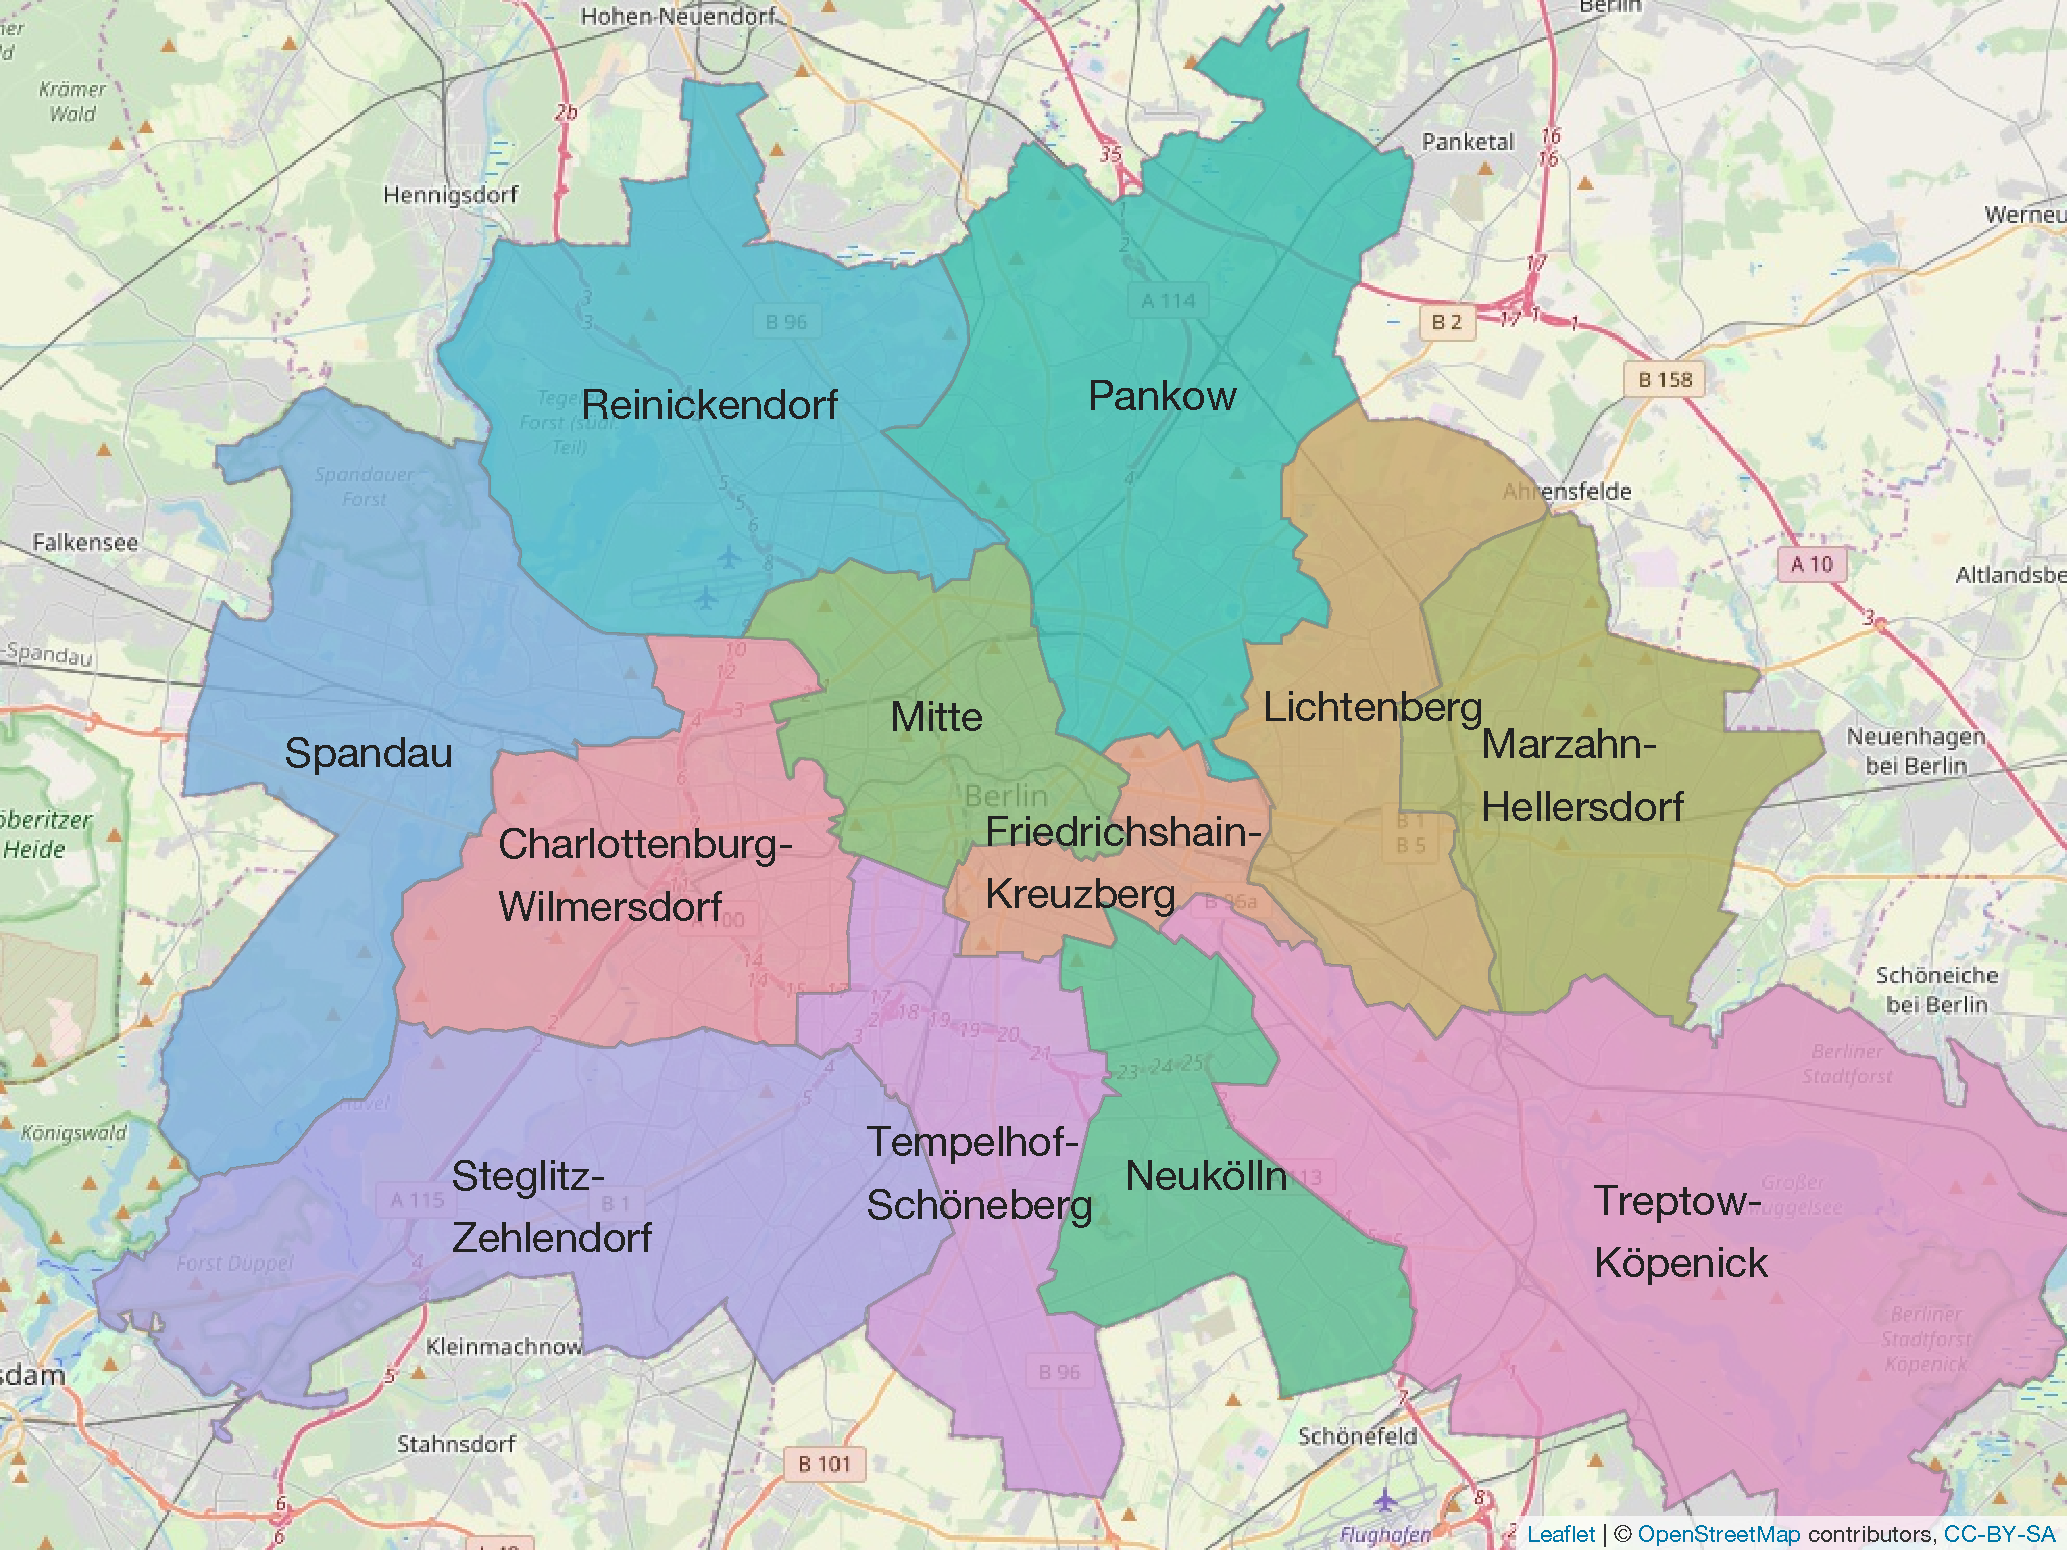
\includegraphics[height=1.8in]{berlin_district_leaflet.pdf}}
\subfloat[With \texttt{ggplot}]{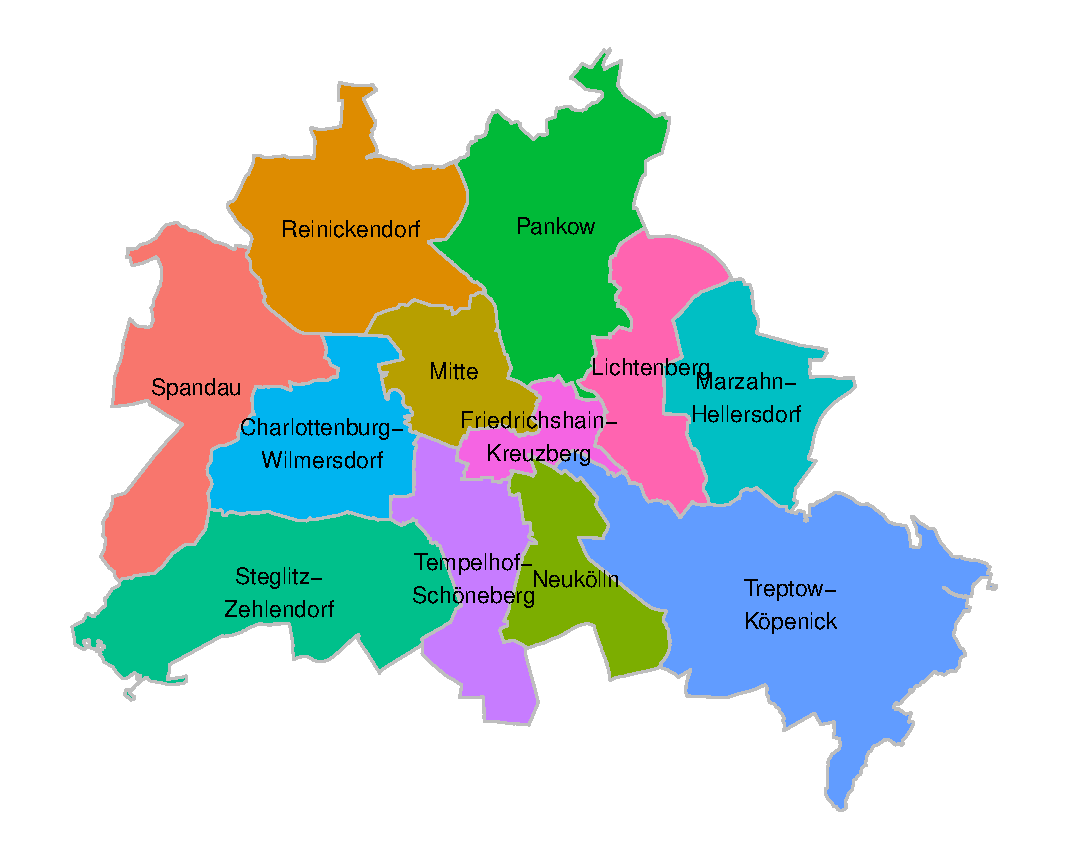
\includegraphics[height=1.8in]{berlin_district_ggplot.pdf}}
\caption{Maps of the Berlin Districts \protect
\includegraphics[scale=0.05]{qletlogo.pdf} {\href{https://github.com/thsis/SPL_WS1718/blob/master/CART/cart_modell_fin.R}{cart\_modell\_fin.R}}}
\centering
\end{figure}

\subsection{Berlin VBB Areas}

The VBB (Verkehrsverbund Berlin-Brandenburg) is "the public transport authority covering the federal states of Berlin and Brandenburg" (CITATION: \href{https://www.vbb.de/en/about-us/the-company-vbb}{VBB Website}). The city of Berlin, in particular, is divided in two fare areas: A, covering the center of Berlin up to the Ringbahn (circular line), and B, from the Ringbahn to the border with Brandenburg. After that there is also the area C, which however will not be covered here since we only consider the city of Berlin.

\begin{figure}[H]
\begin{center}
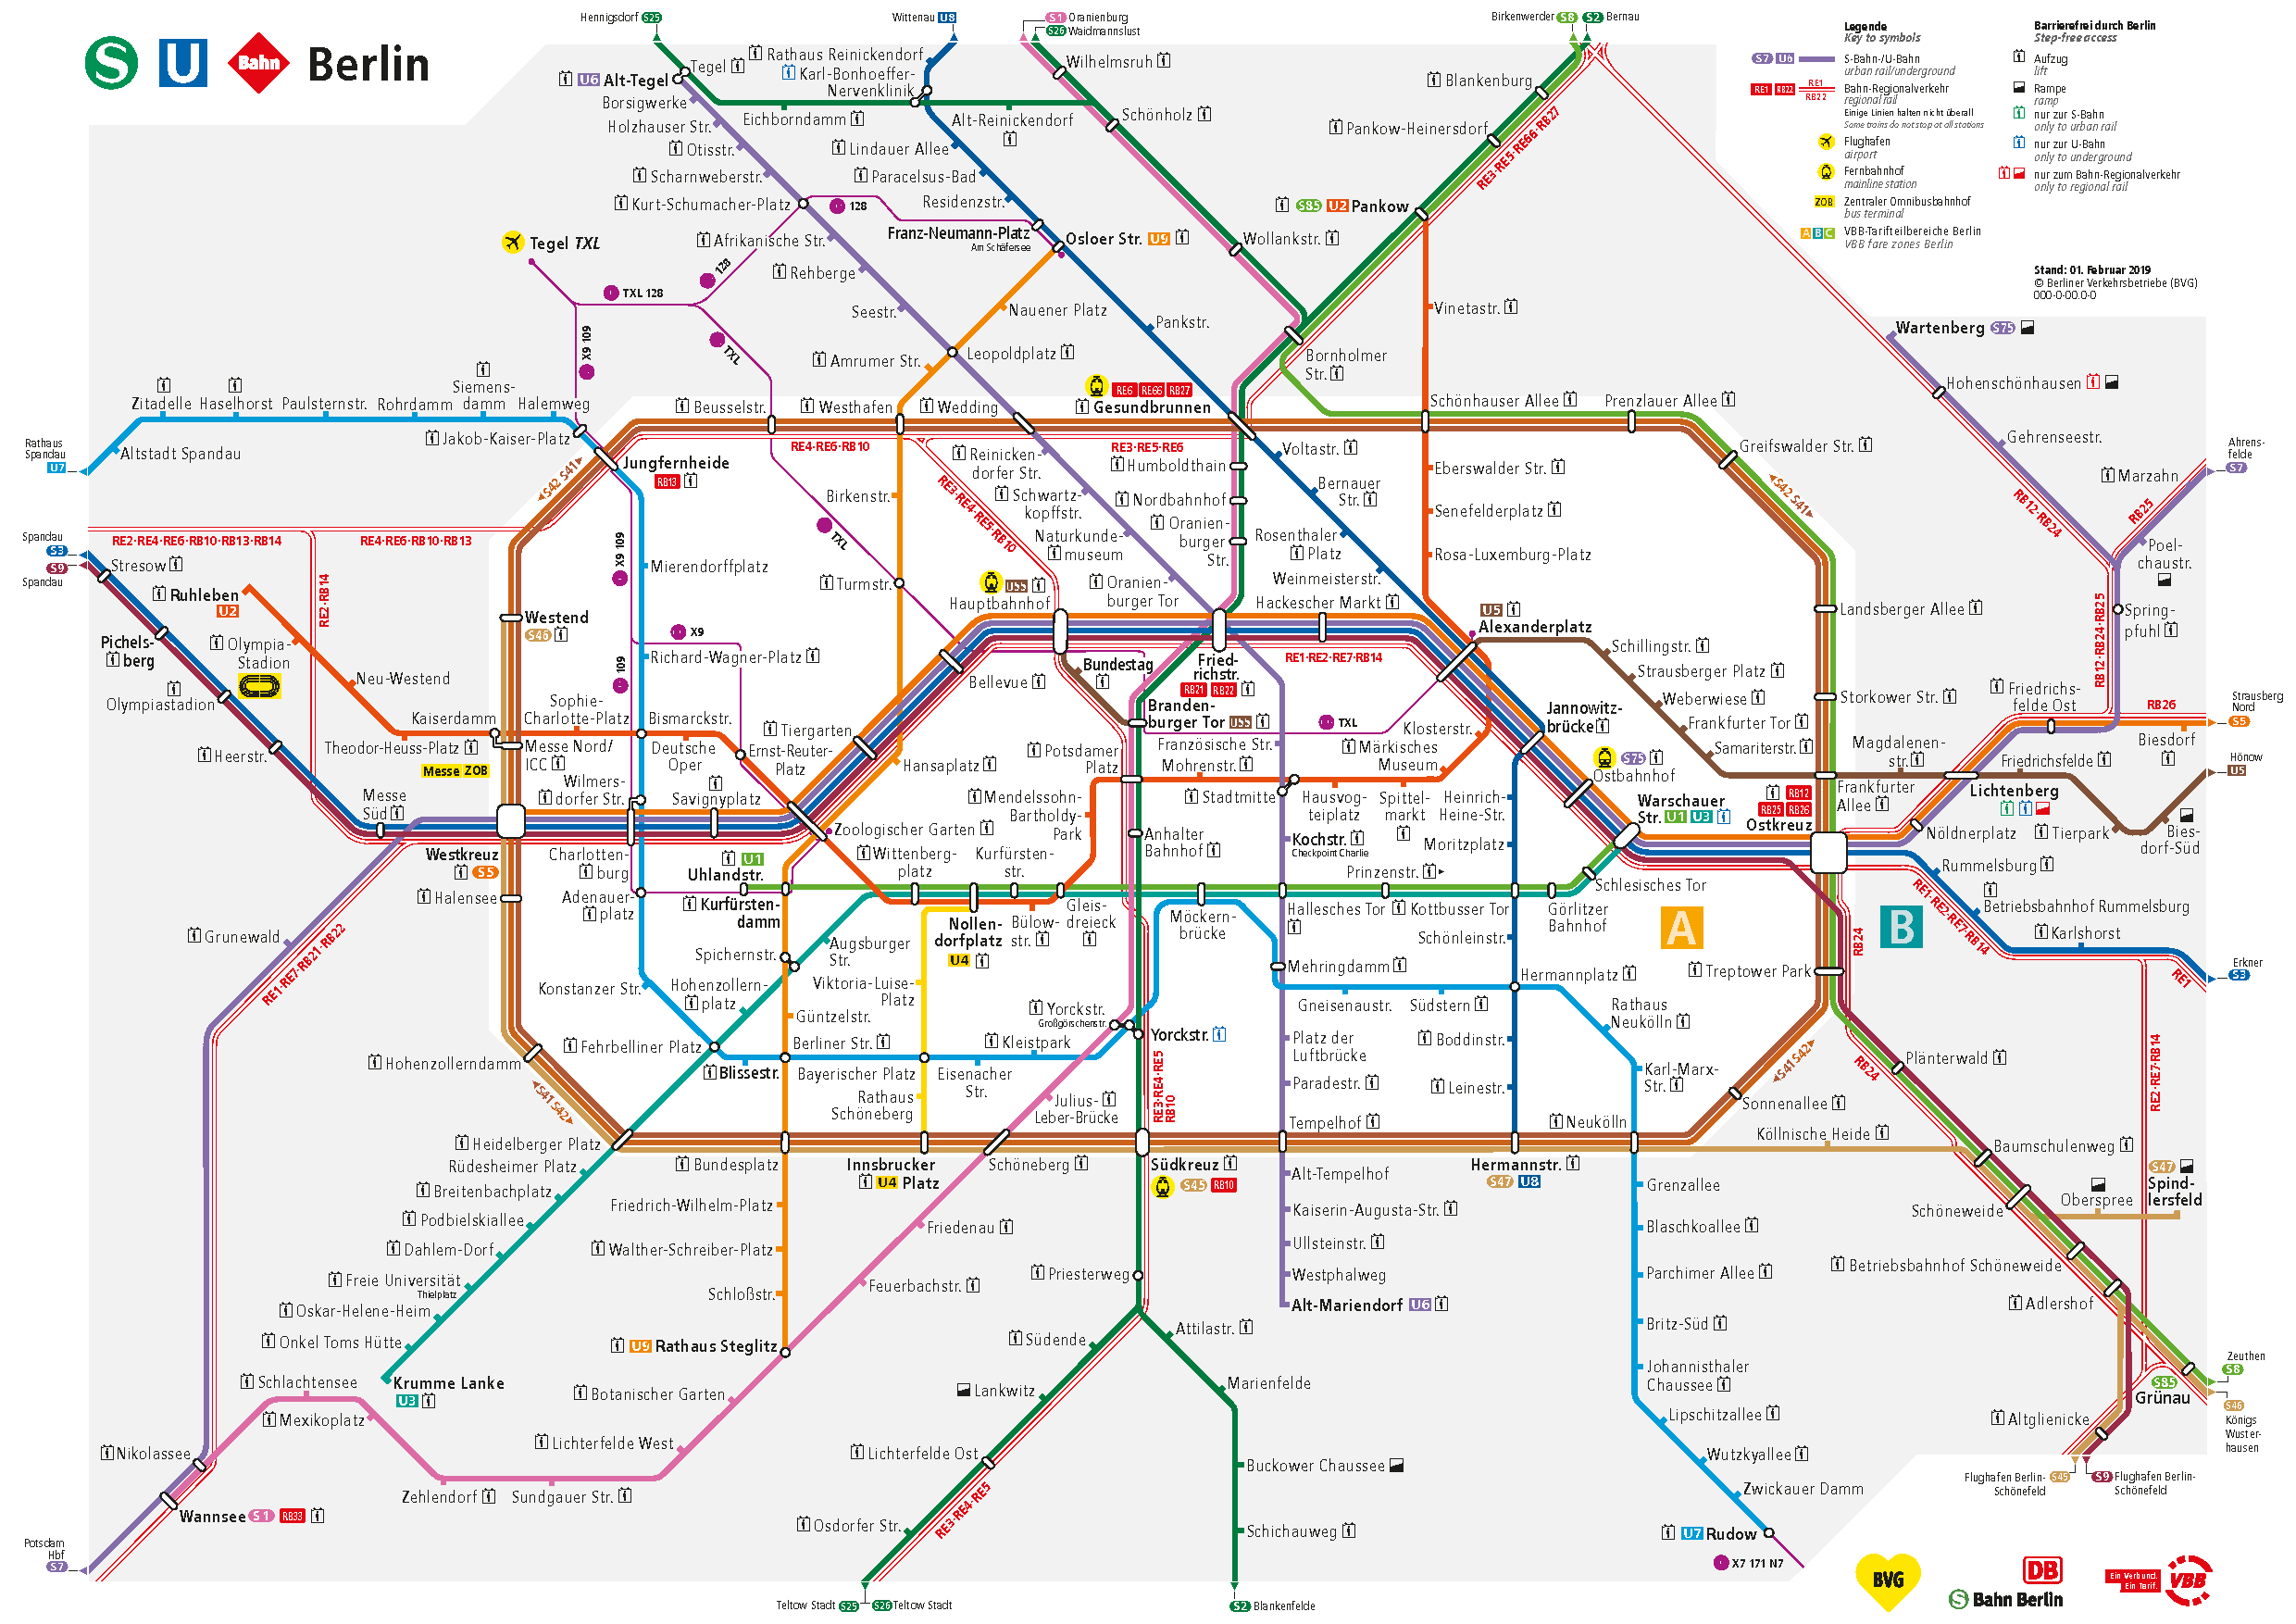
\includegraphics[width=0.8\textwidth, keepaspectratio]{S_und_U-Bahnnetz_mit_Regionalbahn_Innenstadt.pdf} \\
\caption{Network Map of Berlin Areas A and B (from \href{https://www.vbb.de/en/timetables/network-maps}{VBB Website})}
\end{center}
\end{figure}

We tried to replicate these areas by using the Berlin polygons and the stations points, which are again loaded using \texttt{st\_read} from the \texttt{sf} package.

\lstinputlisting[language=R, firstline=18, lastline=19, firstnumber=1, escapechar=|, caption={|\textbf{\href{https://github.com/silvia-ventoruzzo/SPL-WISE-2018/blob/master/Berlin_VBB_Areas/berlin_vbb_areas.R}{berlin\_vbb\_areas.R}}|}]{../Berlin_VBB_Zones/berlin_vbb_zones.R}

First of all, we need to create the polygon for area A. This is done by joining the points and transforming this into a polygon.

Firstly, we filter the stations that belong to the Ringbahn (border of area A). Since the shapefile does not include the line name for the stations, we need to create our own vector of names. We also add the order in which they need to be connected. The first and last station are the same since the circle need to close.

\lstinputlisting[language=R, firstline=22, lastline=33, firstnumber=1, escapechar=|, caption={|\textbf{\href{https://github.com/silvia-ventoruzzo/SPL-WISE-2018/blob/master/berlin_vbb_zones/berlin_vbb_zones.R}{berlin\_vbb\_areas.R}}|}]{../Berlin_VBB_Zones/berlin_vbb_zones.R}

Since some stations appear multiple time, being both subway and lightrail stations (and maybe even bus and tram stops), we filter railway stations, which include both subway and lightrail, and then we calculate the middle point for each station among the ones having the same name.

\lstinputlisting[language=R, firstline=36, lastline=44, firstnumber=1, escapechar=|, caption={|\textbf{\href{https://github.com/silvia-ventoruzzo/SPL-WISE-2018/blob/master/Berlin_VBB_Zones/berlin_vbb_zones.R}{berlin\_vbb\_areas.R}}|}]{../Berlin_VBB_Zones/berlin_vbb_zones.R}

By performing a right join with the dataframe with the Ringbahn station names, we only keep these stations. After performing some preparation steps, we use the function \texttt{st\_polygon} from the \texttt{sf} package, which creates a polygon out of a list of points (CHECK!!!).

\lstinputlisting[language=R, firstline=45, lastline=52, firstnumber=11, escapechar=|, caption={|\textbf{\href{https://github.com/silvia-ventoruzzo/SPL-WISE-2018/blob/master/Berlin_VBB_Zones/berlin_vbb_zones.R}{berlin\_vbb\_areas.R}}|}]{../Berlin_VBB_Zones/berlin_vbb_zones.R}

Secondly we need to create a polygon for entire Berlin. This is done by simply uniting all the neighbourhoods.

\lstinputlisting[language=R, firstline=55, lastline=56, firstnumber=19, escapechar=|, caption={|\textbf{\href{https://github.com/silvia-ventoruzzo/SPL-WISE-2018/blob/master/Berlin_VBB_Zones/berlin_vbb_zones.R}{berlin\_vbb\_areas.R}}|}]{../Berlin_VBB_Zones/berlin_vbb_zones.R}

Finally, we bind the two objects by rows and calculate their intersections thanks to the function \texttt{st\_intersection}. We then define the area names according to how many times the two previous polygons intersect:
	\begin{itemize}
    		\item Area A: where polygons intersect (n. overlaps > 1)
    		\item Area B: where polygons do not intersect (n. overlaps $\leq$ 1)
    \end{itemize}

\lstinputlisting[language=R, firstline=59, lastline=64, firstnumber=21, escapechar=|, caption={|\textbf{\href{https://github.com/silvia-ventoruzzo/SPL-WISE-2018/blob/master/Berlin_VBB_Zones/berlin_vbb_zones.R}{berlin\_vbb\_areas.R}}|}]{../Berlin_VBB_Zones/berlin_vbb_zones.R}

In this code the custom-function \texttt{points\_midpoint} was used to calculate the middle point among many. It extracts the coordinates of the points thanks to \texttt{st\_coordinates} and then calculates the mean of latitude and longitude.

\lstinputlisting[language=R, firstline=2, escapechar=|, caption={|\textbf{\href{https://github.com/silvia-ventoruzzo/SPL-WISE-2018/blob/master//Helpers/points_midpoint.R}{points\_midpoint.R}}|}]{../Berlin_VBB_Zones/Helpers/points_midpoint.R}

This sf object can be used to map the VBB zones using \texttt{leaflet} or \texttt{ggplot2}.

\begin{figure}[H]
\centering
\subfloat[With \texttt{leaflet}]{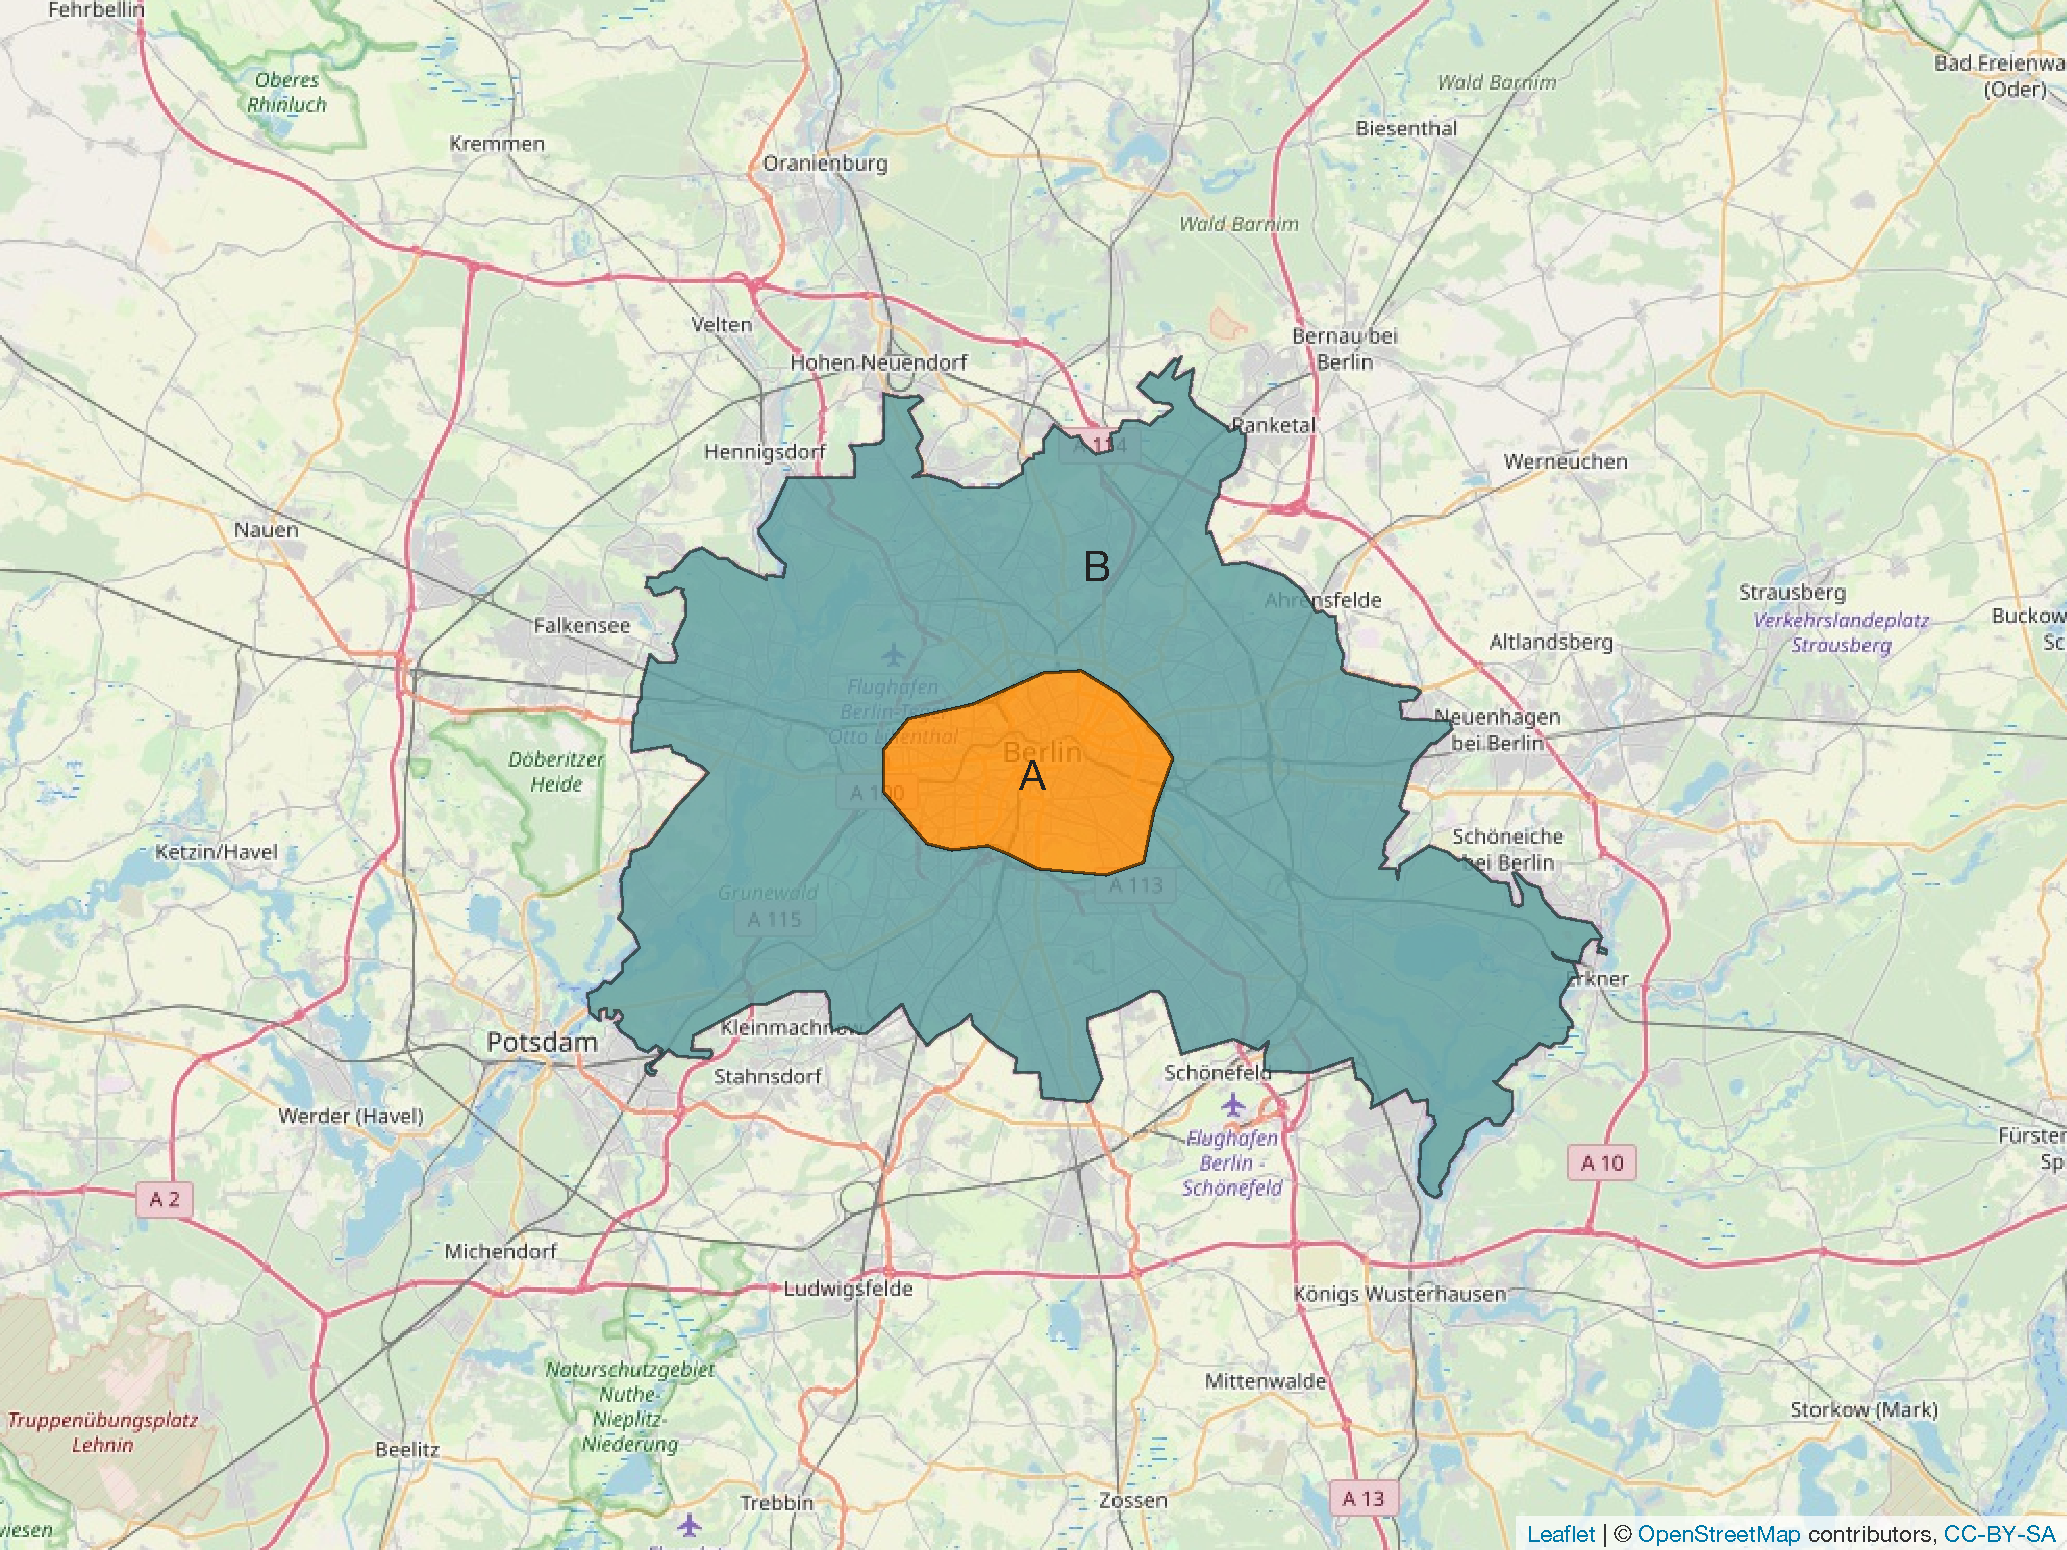
\includegraphics[height=1.8in]{berlin_vbb_zones_leaflet.pdf}}
\subfloat[With \texttt{ggplot}]{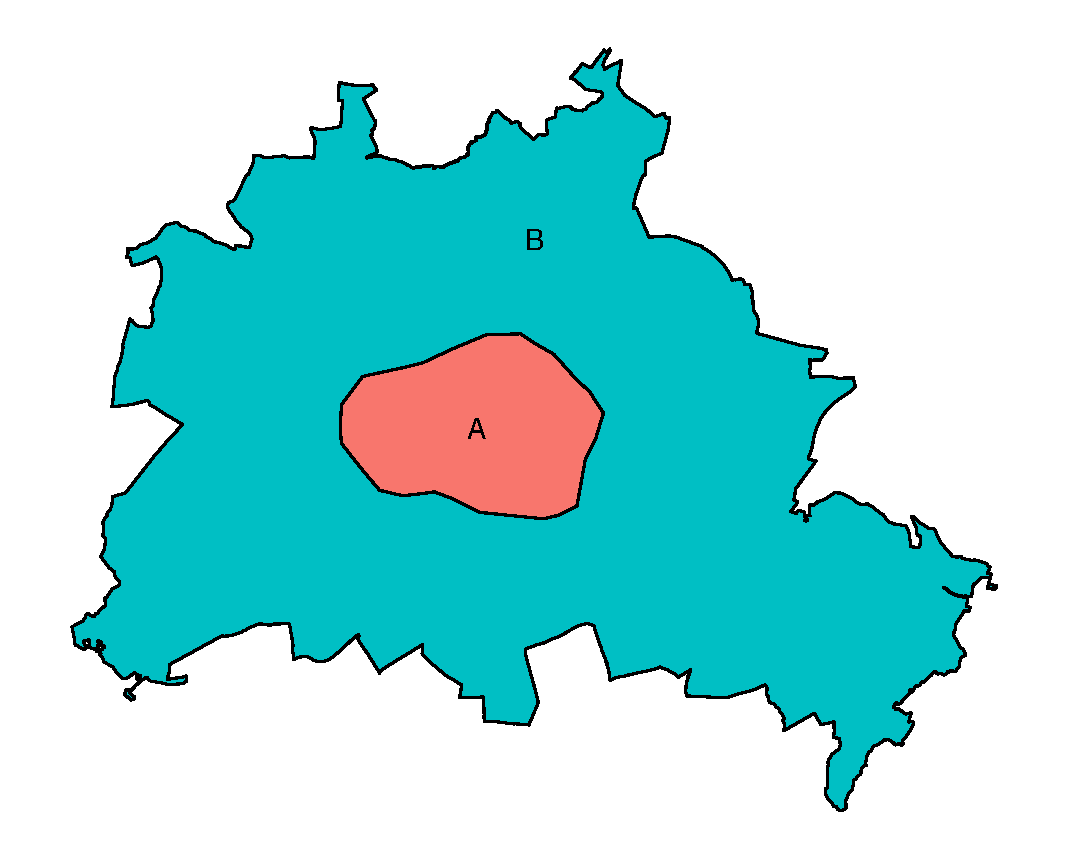
\includegraphics[height=1.8in]{berlin_vbb_zones_ggplot.pdf}}
\caption{Maps of the Berlin VBB Zones}
\centering
\end{figure}

\subsection{airbnb listings' attributes}

The first part of cleaning the airbnb datasets consists in joining the two containing general information according to their common variables and correcting some string values.
Secondly, we proceed in checking for missing values and deriving that information from other correlated variables.
Thirdly, we proceed to feature engineering.
We firstly derive the areas where they are located thanks to the spatial polygons created before and the function \texttt{point\_in\_polygons}.

\lstinputlisting[language=R, firstline=2, escapechar=|, caption={|\textbf{\href{https://github.com/silvia-ventoruzzo/SPL-WISE-2018/blob/master/Helpers/point_in_polygons.R}{point\_in\_polygons.R}}|}]{../Helpers/point_in_polygons.R}

This function loops through the polygons in the \texttt{sf} object and check which points are contained in which polygons. In the end it writes the id associated to the polygon, in our case the area id, in the summary column, which can be named as preferred.

Secondly, for railway stations and tourist attractions we calculate the amount inside a range and the distance to the nearest point using the function \texttt{distance\_count}. In particular, the following parameters will be used:

\begin{itemize}

    \item Railway stations: distance = 1000 (1 km)

    \item (Top 10) attractions: distance = 2000 (2 km)
    
\end{itemize}

\lstinputlisting[language=R, firstline=3, escapechar=|, caption={|\textbf{\href{https://github.com/silvia-ventoruzzo/SPL-WISE-2018/blob/master/Helpers/distance_count.R}{distance\_count.R}}|}]{../Helpers/distance_count.R}

This function firstly calculates the distance between all properties and all reference points, railway stations or tourist attractions, using the Haversine Formula, which "gives  minimum  distance  between  any  two  points  on  spherical body by using latitude and longitude" \citep{haversine:2013}.

\begin{equation}
d = 2r \arcsin \Bigg(\sqrt{\sin^2\Big(\frac{\phi_2 - \phi_1}{2}\Big) + \cos(\phi_2)\cos(\phi_1)\sin^2\Big(\frac{\psi_2 - \psi_1}{2}\Big)}\Bigg)
\end{equation}

%% \mathrm{where} \phi \mathrm{corresponds to the latitude and} \psi \mathrm{to the longitude of the two points.}



\iffalse

\begin{table}[H]
\centering
\begin{tabular}{l}
  \hline
x \\ 
  \hline
id \\ 
  attraction\_count \\ 
  attraction\_dist \\ 
  station\_count \\ 
  station\_dist \\ 
  long \\ 
  lat \\ 
  price \\ 
  property\_type \\ 
  room\_type \\ 
  security\_deposit\_yn \\ 
  cleaning\_fee\_yn \\ 
  host\_is\_superhost \\ 
  accommodates \\ 
  bedrooms \\ 
  beds \\ 
  minimum\_nights \\ 
  review\_scores\_rating \\ 
  number\_of\_reviews \\ 
  reviewed\_yn \\ 
  cancellation\_policy \\ 
  availability\_30 \\ 
  availability\_60 \\ 
  availability\_90 \\ 
  availability\_365 \\ 
  listing\_url \\ 
  district \\ 
  vbb\_area \\ 
  neighbourhood \\ 
  2018\_fall\_availability \\ 
  2018\_winter\_availability \\ 
  2019\_spring\_availability \\ 
  2019\_summer\_availability \\ 
  2019\_fall\_availability \\ 
  2019\_winter\_availability \\ 
   \hline
\end{tabular}
\end{table}

\fi



